\documentclass[a4paper,11pt]{article}
\usepackage{amssymb,epsfig,amsmath,amsthm}
\usepackage{pstricks}
\usepackage{amsmath,amssymb,graphicx}
\usepackage[cm]{fullpage}
%\usepackage[top=1in, bottom=1.25in, left=1.25in, right=1.25in]{geometry}
\usepackage{color}
\usepackage[mathbf,mathcal,text-hat-accent]{euler}
% \usepackage[usenames]{color}
%\usepackage{pdfsync}
%\graphicspath{{Graphix/}}

\title{Machine Learning Nanodegree Project 4 - Training a Smartcab \\ Answers to questions}

\author{Bernhard Langwallner}

\numberwithin{equation}{section}
\numberwithin{figure}{section}
\graphicspath{{Graphix/}}


\renewcommand{\rmdefault}{euler}

\begin{document}
\sffamily
%\baselineskip=18pt plus1pt
\maketitle

%\begin{abstract}
%aaa
%\end{abstract}

\section*{\sffamily Implement a Basic Driving Agent}
\textit{Observe what you see with the agent's behavior as it takes random actions. Does the smartcab eventually make it to the destination? Are there any other interesting observations to note?}

With random actions chosen out of the four available options \textbf{(none, forward, left, right)} the agent reaches the target destination in only a few cases (around 15-20\% according to my trials). The reason for this still significant success rate being that the available time is set quite generous (5 times as many available steps as the $L^1$ norm between origin and destination). As expected the incurred rewards are random, too. Due to many violations of traffic rules, obviously negative rewards are quite frequent (50-60\% according to my trials). Also because of the random nature of the agent's trajectory it does not necessarily travel very far on a single trip, it often keeps in a smaller neighborhood of its origin.\\
An interesting observation with implications for training later on is the following: Since there are only few other agents in the grid, the learning agent rarely meets other agents. This means that the agent's learning progress should be quite good on states that only involve a traffic light status and the learning agent's target direction of travel (no other traffic). So the agent should quickly learn to travel in the right direction based on the traffic light status.


\section*{\sffamily Inform the Driving Agent}
\textit{What states have you identified that are appropriate for modeling the smartcab and environment? Why do you believe each of these states to be appropriate for this problem?}

I have chosen the four following variables to make up the state variable: \textbf{traffic light status, oncoming traffic action, left traffic action, next waypoint}. Traffic light status is obvious as it represents a key aspect of abiding by traffic rules. Oncoming as well as left traffic action are also important to observe as their presence limit the agent's permitted actions (see defined traffic rules). I omitted right traffic action because in either traffic light setting cars from the right are irrelevant. Sparing this variable also means the dimension of the state space is smaller and therefore training can be accelerated. \\
Finally, next waypoint is the one piece of information we need to encode the agent's desired direction of travel. \\ \\


\textit{How many states in total exist for the smartcab in this environment? Does this number seem reasonable given that the goal of Q-Learning is to learn and make informed decisions about each state? Why or why not?}

We can calculate the number of possible states as follows: we have two possible traffic lights settings (green, red), 4 oncoming traffic actions (none, forward, left, right), 4 similar left traffic actions and three possible next waypoints (forward, left, right). Hence, the number of states is:
\begin{equation*}
\mathsf{\# States} = 2  \times 4 \times 4 \times 3 = 96.
\end{equation*}
However, we need to keep in mind that in Q-learning we are training the Q-matrix for (state, action) pairs. Since there are 4 actions (None, forward, left, right) we get 384 Q-matrix elements. This is a number of elements that is possible to train with several test runs. Note that as stated earlier, many of the (state, action) pairs are rarely visited: in particular those involving other cars. I would expect that with 20-30 training runs (30-40 steps each) we get to a solid understanding of the Q-matrix (given the parameters are tuned to some degree).


\section*{\sffamily Implement a Q-Learning Driving Agent}
\textit{What changes do you notice in the agent's behavior when compared to the basic driving agent when random actions were always taken? Why is this behavior occurring?}

The changes when going from the uninformed random behavior to Q-learning occur quite fast. After a handful of trials we can already observe how the agent is drawn to the destination. It clearly starts following the path that is suggested by next waypoint in every step. Particularly in situations that do not involve any other cars (otherwise empty crossings) the agent seems to follow next waypoint well while obeying the traffic rules in most cases. In situations with other cars at the crossing the agent still sometimes derailed from the ideal path. This is unsurprising as learning in these rarer situations happens less frequently and therefore overall more slowly. However, the agent manages to get back on track quickly.

The reason for this continuously changing (improving) behavior simply is that we have a feedback loop in place. From a random world to start with we continuously encode rewards into the Q-matrix. Since the values of the q-matrix determine the next action, the agent will start choosing actions that promise more reward.

\section*{\sffamily Improve the Q-Learning Driving Agent}
\textit{Report the different values for the parameters tuned in your basic implementation of Q-Learning. For which set of parameters does the agent perform best? How well does the final driving agent perform?}

We will look at the parameters one at a time. In my experiments, it looked like the precise value of $\gamma$ was relatively unimportant. Only in cases with large constant learning factor $\alpha$ it looked like a $\gamma$ closer to $1$ than $0$ was required to balance the reward term $R(s,a,s')$. However, with larger $\alpha$ reliable learning progress is difficult to obtain.

The parameter $\varepsilon$ (the probability of taking a random step) is introduced so the agent is more likely to visit new states, which is important to train as many Q-matrix elements as possible. As recommended I chose decaying $\varepsilon$. Comment: for reasonable values of $\alpha$ and $\gamma$ decent success rate can be obtained if $\varepsilon$ is chosen constant but small, e.g. $\varepsilon=0.1$.

My choice of $\varepsilon$ had the following form: $\varepsilon_k = \varepsilon_0^k$ where $k$ is the number of steps of the agent (cumulated over a number of trials). Here are a few learnings from observing different values of $\varepsilon_0$ (while leaving $\alpha=0.1$ and $\gamma=0.1$ constant). Solid success rates can be obtained for most values of $\varepsilon_0$, even for small values like, say, $0.5$. However, it seems that this type of value makes learning less reliable. Every now and again, very low success rates on 100 trial runs are obtained. This may have to do with the fact that only few Q-matrix elements are properly trained due to lack of enough randomness at the beginning of the training phase. I finally found values of $\varepsilon_0>0.95 $ to work quite well. As a reference point: for $\varepsilon_0=0.99$ after $k\approx 230$ steps $\varepsilon$ reaches $0.1$. This seems a good value given the above calculated number of Q-matrix elements.

Finally, the learning parameter $\alpha$ turns out to be quite important. For large values of $\alpha > .9$ learning basically did not occur. When $\alpha\approx 0.5$, learning was very unreliable (heavily varying success rates). For smaller values of $\alpha \approx 0.1$ learning did occur quite reliably with good success rates $>80-90\%$. However, it seemed reasonable to also choose $\alpha_k = c_\alpha\alpha_0^k$ decaying with $c_\alpha=.2$ for example. Here, $\alpha_0$ can be chosen very close to $1$, e.g., $\alpha_0=0.999$ to ensure learning happens over a longer time horizon.

To summarize, the following values turned out to work well ($k$ being the iterator over steps)
\begin{equation*}
\varepsilon_k =  0.99^k, \ \ \ \gamma_k = 0.1,\ \ \ \alpha_k = 0.2\times 0.999^k.
\end{equation*}
With these values the success rate of 100 subsequent trials was consistently $90\%$ or higher (always including the initial, training-heavy phase). 

One more word about initialization of the Q-matrix: I found that using random values for initialization ensures the agent explores more states in its early learning stage. As pointed out in the first review, it is beneficial to use somewhat larger values for initialization makes sure that exploration is possible beyond the first incurred positive reward of $2$ (optimistic initialization). Therefore, I initialize all Q-matrix values with $Q(\mathsf{state, action}) = 2.0 + \mathsf{random\ value\ in\ } [0, 1]$
\\ \\

\textit{Does your agent get close to finding an optimal policy, i.e. reach the destination in the minimum possible time, and not incur any penalties? How would you describe an optimal policy for this problem?}

As reported in the previous question, after tuning the parameters to some degree, success rates were quite good. Especially after the initial, say, 15-20 runs, the large majority of trial runs ended in success. Still, in a significant share of steps, negative rewards were incurred, on average around $\approx 10\%$ (always for 100 subsequent runs; this number decreases slightly as we run more trials in succession). In the later stages, the agent occasionally ran a red traffic light, thus incurring a small negative reward. So in that sense the final policy was not optimal. (Comment: there may be a point in tuning the rewards, too. For example, heavier negative rewards for running a red light).

As to the time required to reach the destination, I found that for 100 subsequent trial runs the agent on average needed around $50-55\%$ of the allowed number of steps given by the specified deadline (five times the distance). Factoring in traffic, traffic lights etc. this seems sensible. 

Obviously, the optimal policy depends on the choice of the model, including parameters like the rewards. In this simple model, the agent gets a reward of $2$ if it follows the next waypoint suggestion. So in this case, the optimal policy would likely always pick the next waypoint if admissible by traffic rules or else stall if next waypoint was forbidden by traffic rules/traffic lights.

This would possibly change a little if (more realistically) the agent was rewarded for reducing the distance to the destination. If I want to go from $(0,0)$ to $(2,2)$, it is irrelevant whether the next step is to $(1,0)$ or $(0,1)$. However, in our model only one of the would count as next waypoint and therefore come with a reward. 

\begin{figure*}
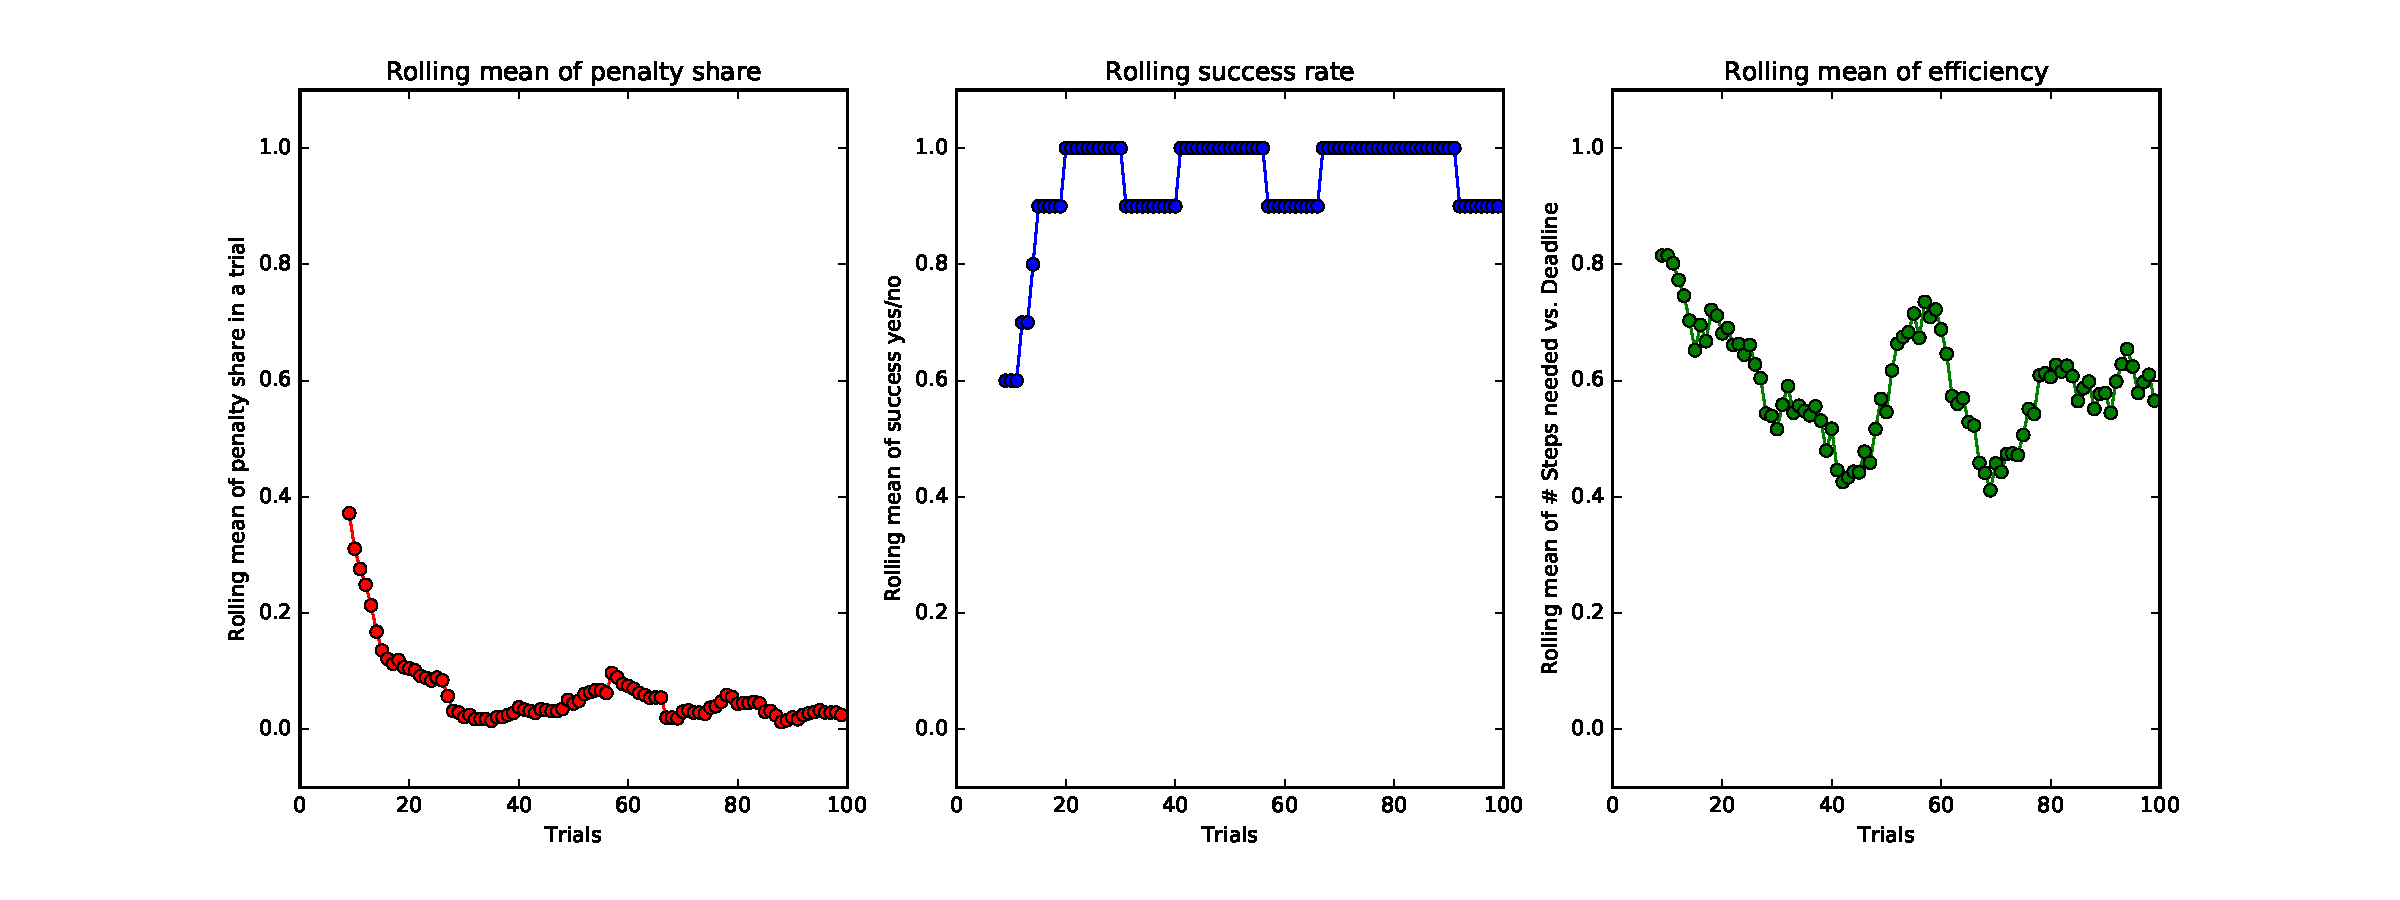
\includegraphics[width=0.98\textwidth]{charts}
\caption{Different KPIs for an example run of 100 trials}
\end{figure*}


\end{document}